\chapter{Analýza časových řad}

\section{Náhodnost časových řad}

Jednou z podmínek OLS je náhodnost výběru, který slouží pro 
odhad regresního modelu. Na realizovanou časovou posloupnost lze pohlížet jako na posloupnost 
náhodných veličin indexovaných časem, tj. jako na realizaci 
určitého stochastického procesu. Proto předpoklad náhodnosti splňují i časové řady.

\section{Příklady regresních modelů časových řad}

\subsection{Statický model}

Uvažujme statický model
\begin{equation}
	y_t = \beta_0 + \beta_1 z_t + u_t, ~~~ t = 1, 2, ..., n,
\end{equation}
který modeluje okamžitou vazbu mezi $y$ a $z$. Statický model 
aplikujeme v případě, kdy věříme, že změna $z$ v čase $t$ má 
okamžitý dopad na $y$. Výše uvedený model je jednofaktorový, 
nicméně základní myšlenku lze snadno zobecnit také na 
vícefaktorový model.

\subsection{Model s konečným rozdělením zpoždění}

V modelu s konečným rozdělením zpoždění [finite distributed lag (FDL) model] je jedna nebo více 
nezávislých proměnných zpožděných o konečný počet kroků. 
Model má tedy např. tvar
\begin{equation}
	y_t = \beta_0 + \beta_1 z_t + \beta_2 z_{t - 1} + \beta_3 z_{t - 2} 
	+ u_t.
\end{equation}
To, že výše uvedený model obsahuje současně $z_t$, $z_{t - 1}$ i 
$z_{t - 2}$, lze interpretovat tak, že případný šok v systému ``rezonuje'' určitou dobu, než zcela odezní. Pro ilustraci předpokládejme, že
\begin{equation}
	..., z_{t - 2} = c, z_{t - 1} = c, z_t = c + 1, z_{t + 1} = c, z_{t 
	+ 2} = c , ...,
\end{equation}
což implikuje
\begin{equation}
	y_{t - 1} = \alpha_0 + \delta_0 c + \delta_1 c + \delta_2 c,
\end{equation}
\begin{equation}
	y_t = \alpha_0 + \delta_0(c + 1) + \delta_1 c + \delta_2 c,
\end{equation}
\begin{equation}
	y_{t + 1} = \alpha_0 + \delta_0 c + \delta_1 (c + 1) + \delta_2 c,
\end{equation}
\begin{equation}
	y_{t + 2} = \alpha_0 + \delta_0 c + \delta_1 c + \delta_2 (c + 1),
\end{equation}
\begin{equation}
	y_{t + 3} = \alpha_0 + \delta_0 c + \delta_1 c + \delta_2 c.
\end{equation}
Parametr $\delta_0 = y_t - y_{t - 1}$, který měří okamžitý dopad 
změny z $c$ na $c + 1$ v čase $t$, nazýváme propenzitním účinkem 
(impact propensity). Podobně lze také interpretovat $\delta_1 = y_{t 
+ 1} - y_{t - 1}$ a $\delta_2 = y_{t + 2} - y_{t - 1}$.

Pokud bychom namísto dočasných změn uvažovali změny trvalé, tj.
\begin{equation}
	y_{t - 1} = \alpha_0 + \delta_0 c + \delta_1 c + \delta_2 c,
\end{equation}
\begin{equation}
	y_t = \alpha_0 + \delta_0(c + 1) + \delta_1 c + \delta_2 c,
\end{equation}
\begin{equation}
	y_{t + 1} = \alpha_0 + \delta_0 (c + 1) + \delta_1 (c + 1) + \delta_2 c,
\end{equation}
\begin{equation}
	y_{t + 2} = \alpha_0 + \delta_0 (c + 1) + \delta_1 (c + 1) + \delta_2 (c + 1),
\end{equation}
pak součet $\delta_0 + \delta_1 + \delta_2$ představuje dlouhodobou změnu 
$y$ při trvalé změně $z$ a nazýváme ho dlouhodobou propenzitou 
(long-run propensity).

Obecný model s konečným rozdělením zpoždění řádu $q$ má tvar
\begin{equation}
	y_t = \alpha_0 + \delta_0 z_t + \delta_1 z_{t - 1} + ... + \delta_q 
	z_{t - q} + u_t
\end{equation}
s dlouhodobou propenzitou $\delta_0 + \delta_1 + ... + \delta_q$.

Z důvodu časté korelace mezi jednotlivými zpožděnými $z$, 
tj. multikolinearitě v regresním modelu, může být obtížné 
získat přesné odhady jednotlivých parametrů $\delta_j$. Nicméně, 
ačkoliv je odhad $\delta_j$ problematický, lze často získat dobrý 
odhad dlouhodobé propenzity modelu.

\section{OLS vlastnosti konečného výběru}

\subsection{Nestrannost OLS}

\begin{assumption}[TS.1 - lineární model]
Stochastický proces ${(x_{t1}, x_{t2}, ..., x_{t3}, y_t): t = 1, 2, 
..., n}$ sleduje lineární model
\begin{equation}
y_t = \beta_0 + \beta_1 x_{t1} + ... + \beta_k x_{tk} + u_t,
\end{equation}
kde ${u_t: t = 1, 2, ..., n}$ představuje chybovou posloupnost. 
Parametr $n$ představuje počet pozorování, tj. délku časové řady.

\raggedleft{$\clubsuit$}
\end{assumption}

\begin{assumption}[TS.2 - neexistence perfektní kolinearity]
V náhodném výběru (a tím pádem také v podkladovém stochastickém 
procesu) není žádná z nezávislých veličin konstantní a 
žádná z nezávislých veličin není lineární kombinací zbývajících.

\raggedleft{$\clubsuit$}
\end{assumption}

\begin{assumption}[TS.3 - nulová střední hodnota]
Pro dané hodnoty nezávislých veličin je střední hodnota 
chyby $u_t$ nulová, tj.
\begin{equation}
E[u_t | X] = 0, ~~~ t = 1, 2, ..., n.
\end{equation}


\raggedleft{$\clubsuit$}
\end{assumption}

Výše uvedený předpoklad je mimo jiné podmíněn správnou 
specifikací lineárního regresního modelu, který popisuje vztah mezi 
$y$ a nezávislými veličinami. Jestliže je $u_t$ nezávislé na 
$X$ a $E[u_t] = 0$, pak je předpoklad TS.3 automaticky splněn.

Pokud
\begin{equation}
E[u_t|x_{t1}, ..., x_{tk}] = E[u_t | x_t] = 0,
\end{equation}
říkáme, že $x_{tj}$ je souběžně exogenní (comtemporaneous 
exogenous), což implikuje $cor[x_{tj}, u_t] = 0$. Předpoklad TS.3 
však vyžaduje více než jen souběžnou exogennost - chyba $u_t$ 
musí být nekorelovaná s $x_{sj}$ i pro $s \ne t$. V tomto případě 
říkáme, že nezávislé proměnné jsou striktně exogenní (strictly exogenous). 
Striktní exogennost je nezbytná pro nestrannost OLS. Je však 
důležité zdůraznit, že TS.3 neklade žádná omezení pro 
vzájemnou korelaci náhodných veličin či pro korelaci chyby $u_t$ v 
čase.

Uvažujme regresní model
\begin{equation}
y_t = \beta_0 + \beta_1 z_t + u_t.
\end{equation}
Předpoklad TS.3 vyžaduje nejen neexistenci korelace mezi $u_t$ a 
$z_t$, ale také neexistenci korelace mezi $u_t$ a všemi minulými a 
budoucími hodnotami $z$., což má dva následky. Za prvé, 
regresní model vysvětlující chování $y$ by neměl zahrnovat 
zpožděná (lagged) $z$. Za druhé, dnešní změny chyby $u_t$ by 
neměly mít vliv na budoucí změny $z$. Pro ilustraci uvažujme model 
počtu vražd na tisíc obyvatel jako funkci počtu policistů na 
tisíc obyvatel, tj.
\begin{equation}
mrdrte_t = \beta_0 + \beta_1 polpc_t + u_t.
\end{equation}
Je přirozené předpokládat, že $u_t$ je nekorelované s aktuální 
nebo dokonce minulou velikostí policejního sboru. Nicméně 
předpokládejme, že město upravuje jeho velikost dle počtu vražd v 
minulosti. Protože vyšší $u_t$ znamená vyšší počet vražd, je 
$polpc_{t + 1}$ korelováno s $u_t$. Předpoklad TS.3 je tak porušen.

Podobné úvahy jsou relevantní také v případě modelu se zpožděním. 
Nicméně obvykle nepředstavuje problém korelace mezi $u_t$ a 
minulými hodnotami $z$, protože v regresním modelu máme minulá $z$ 
``pod kontrolou''. Nicméně vliv chyby $u$ na budoucí hodnoty $z$ je 
problémem vždy.

Striktně exogenní vysvětlující veličiny nereagují na minulé hodnoty $y$ - např. objem srážek v daném roce 
nemůže být ovlivněn výší zemědělské produkce v minulém roce. 
Nicméně některé nezávislé veličiny, jako např. míra 
mechanizace v zemědělství, nemusí být striktně exogenní a její 
míra může být dána výší zemědělské produkce v předchozím roce.
To je typický problém sociálních věd, kde mnoho nezávislých veličin 
porušuje předpoklad striktní exogenity.

\begin{theorem}[Nestrannost OLS odhadů]
Při splnění předpokladů TS.1, TS.2 a TS.3 jsou OLS odhady 
nestranné a to jak podmíněně na $X$, tak nepodmíněně.
\begin{equation}
E[\hat{\beta_j}] = \beta_j, ~~~ j = 0, 1, ..., k
\end{equation}

\raggedleft{$\clubsuit$}
\end{theorem}

Důkaz této věty je ve své podstatě totožný s důkazem věty 3.1 
v kapitole 3, a proto jej vynecháme. Také analýza zkreslení z 
titulu vynechání relevantní nezávislé veličiny, kterou jsme 
diskutovali v kapitole 3, je pro časové řady totožná.

\subsubsection{Rozptyl OLS dohadů a Gaus-Markovova věta}

\begin{assumption}[TS.4 - homoskedasticita]
Rozptyl chyby $u$ podmíněný $X$ je shodný pro všechna $t$, tj.
\begin{equation}
var[u_t|X] = var[u_t] = \sigma^2_t, ~~~ t = 1, 2, ..., n.
\end{equation}

\raggedleft{$\clubsuit$}
\end{assumption}

Pro ilustraci uvažujme vývoj úrokových sazeb, který je do značné míry 
ovlivňován chováním centrální banky. Protože se toto chování 
mění s tím, jak se vyvíjí politika centrální banky, je výše uvedený 
předpoklad v tomto konkrétním případě velmi pravděpodobně porušen.

\begin{assumption}[TS.5 - neexistence sériové korelace aka autokorelace]
Libovolné dva chybové členy podmíněné $X$ jsou vzájemně nekorelované, tj.
\begin{equation}
corr[u_t, u_s|X] = 0, ~~~ \text{pro všechna} ~ t \ne s.
\end{equation}

\raggedleft{$\clubsuit$}
\end{assumption}

Nejjednodušší způsob, jak tento předpoklad uchopit, je ignorovat 
podmíněnost na $X$. Pak se předpoklad TS.5 zjednoduší na
\begin{equation}
corr[u_t, u_s] = 0, ~~~ \text{pro všechna} ~ t \ne s.
\end{equation}

Uvažujme ilustrativní případ dvou po sobě jdoucích chyb. 
Konkrétně uvažujme, že pokud $u_{t-1} > 0$, 
pak v průměru taktéž platí $u_t > 0$. V tomto případě zcela 
zřejmě vykazují chybové členy autokorelaci, tj. $corr[u_t, u_{t - 
1}] > 0$. Vraťme se opět k výše uvedenému příkladu vývoje 
úrokových sazeb. V našem kontextu to znamená, že pokud jsou jednu 
časovou periodu úrokové sazby nečekaně vyšší, lze 
předpokládat, že budou vyšší také následující časovou 
periodu. Toto je bohužel typická charakteristika chování chybového 
členu pro mnoho časových řad, se kterými se v praxi setkáváme.

Je důležité si uvědomit, že předpoklad TS.5 nám nezakazuje 
autokorelaci nezávislých veličin. Například míra inflace, která 
bude velice pravděpodobně důležitou vysvětlující veličinou pro 
vývoj úrokových sazeb, je typicky silně autokorelovaná.

Přirozenou otázkou je, proč jsme se v kapitolách 3 a 4 také nezaobírali 
problematikou autokorelace tak, jak je tomu v případě časových 
řad. Na rozdíl od časových řad totiž byla nezávislost $u_i$
 a $u_h$ pro jim odpovídající pozorování $i$ a $h$ zajištěna 
 předpokladem náhodného výběru. Lze totiž dokázat, že pro 
 náhodný výběr jsou chyby dvou rozdílných pozorování při 
 jejich podmínění na $X$ nezávislé. Problém autokorelace tak 
 zůstává omezen na časové řady.

\begin{theorem}[Výběrový rozptyl OLS odhadů]
Nechť jsou splněny předpoklady TS.1 až TS.5 označované též jako 
Gaus-Markovovy předpoklady. Pak je rozptyl odhadu $\hat{\beta}_j$ 
podmíněný $X$ dán vztahem
\begin{equation}
var[\hat{\beta}_j | X] = \frac{\sigma^2}{SST_j(1 - R^2_j)}, ~~~ j = 1, 
..., k,
\end{equation}
kde $SST_j$ je celkový součet čtverců nezávislé veličiny 
$x_{tj}$ a $R^2_j$ je získán z regresního modelu, 
který vysvětluje $x_j$ pomocí zbývajících nezávislých veličin.

\raggedleft{$\clubsuit$}
\end{theorem}

\begin{theorem}[Nestrannost odhadu $\sigma^2$]
Při splnění předpokladů TS.1 až TS.5 je odhad
\begin{equation}
\hat{\sigma}^2 = \frac{SSR}{df}
\end{equation}
nestranným odhadem $\sigma^2$, kde $df = n - k - 1$.

\raggedleft{$\clubsuit$}
\end{theorem}

\begin{theorem}[Gaus-Markovova věta]
Při splnění předpokladů TS.1 až TS.5 jsou OLS odhady podmíněné 
$X$ nejlepšími nezkreslenými lineárními (BLUE) odhady.

\raggedleft{$\clubsuit$}
\end{theorem}

\subsubsection{Testování hypotéz}

\begin{assumption}[TS.6 - normalita]
Chyby $u_t$ jsou nejen nezávislé na $X$, ale jsou také vzájemně 
nezávislé a sledují standardní normální rozdělení, tj. 
\begin{equation}
u_t \sim N[0, 1].
\end{equation}

\raggedleft{$\clubsuit$}
\end{assumption}

Splnění předpokladu TS.6 implikuje splnění předpokladů TS.3, 
TS.4 a TS.5. Tento předpoklad je však silnější, protože navíc 
vyžaduje vzájemnou nezávislost a normalitu chybových členů regresního modelu.

\begin{theorem}[Normální výběrové rozdělení]
Při splnění předpokladů TS.1 až TS.6, jsou OLS odhady, 
podmíněně na $X$, normálně rozdělené. Dále v případě nulové 
hypotézy sleduje každá $t$ statistika $t$ rozdělení a každá $F$ 
statistika $F$ rozdělení. Obvyklý postup pro konstrukci intervalů 
spolehlivosti je tak rovněž platný.

\raggedleft{$\clubsuit$}
\end{theorem}

\subsection{Funkcionální forma a binární veličiny}

\subsubsection{Funkcionální forma}

Všechny funkcionální formy, které jsme diskutovali v předchozích 
kapitolách, lze aplikovat také na časové řady. Pravděpodobně 
nejvýznamnější je přirozený logaritmus, protože časové řady s 
konstantní relativní změnou jsou v praxi poměrně běžné.

Přirozený logaritmus lze také použít pro modely s konečným rozdělením
zpoždění. Pro ilustraci předpokládejme, že poptávka po 
penězích a hrubý domácí produkt jsou provázány následujícím způsobem.
\begin{multline}
\log(M_t) = \alpha_0 + \delta_0 log(GDP_t) + \delta_1 log(GDP_{t - 
1})\\
+ \delta_2 \log(GDP_{t - 2}) + \delta_3 \log(GDP_{t - 3}) + u_t
\end{multline}
Propenzitní účinek $\delta_0$ nazýváme krátkodobou elasticitou; 
propenzitní účinek $\delta_0 + \delta_1 + \delta_2 + \delta_3$ pak
nazýváme dlouhodobou elasticitou.

\subsubsection{Binární veličiny}

V časových řadách lze také použít binární veličiny, které 
indikují, zda-li v dané časové periodě nastala či nenastala 
určitá událost. V praxi jsou binární veličiny velmi často 
používány k izolování časových period, které mohou 
být z nejrůznějších důvodů odlišné od ostatních dat.

Binární veličiny jsou taktéž klíčem k tzv. případové studii 
(event study), jejímž cílem je zjistit, zda-li má určitá událost 
dopad na výsledek, či nikoliv. Typickým příkladem případové 
studie jsou analýzy efektivnosti akciových trhů.

\subsection{Časové trendy a sezónnost}

\subsubsection{Časové trendy}

Některé řady obsahují časový trend. Pokud bychom ignorovali 
skutečnost, že dvě časové posloupnosti sledují stejný nebo opačný 
trend, mohli bychom dojít k mylnému závěru, že změny jedné 
veličiny jsou způsobeny změnami jiné veličiny. V řadě případů 
se totiž dvě časové posloupnosti mohou zdát korelované pouze 
proto, že sledují podobný trend, ačkoliv spolu zjevně nesouvisí.

Jaký statistický model je vhodný pro podchycení trendu v časové 
řadě? Jeden z populárních modelů má tvar
\begin{equation}
y_t = \alpha_0 + \alpha_1t + e_t, ~~~ t = 1, 2, ...,
\end{equation}
kde, ve své nejjednodušší podobě, je ${e_t}$ nezávislá 
posloupnost sledující identické pravděpodobnostní rozdělení s 
$E[e_t] = 0$ a $var[e_t] = \sigma^2_e$. Všimněme si, že člen 
$\alpha_1 t$ ve výše uvedené rovnici představuje lineární časový trend.

\begin{figure}[htp]
\centering
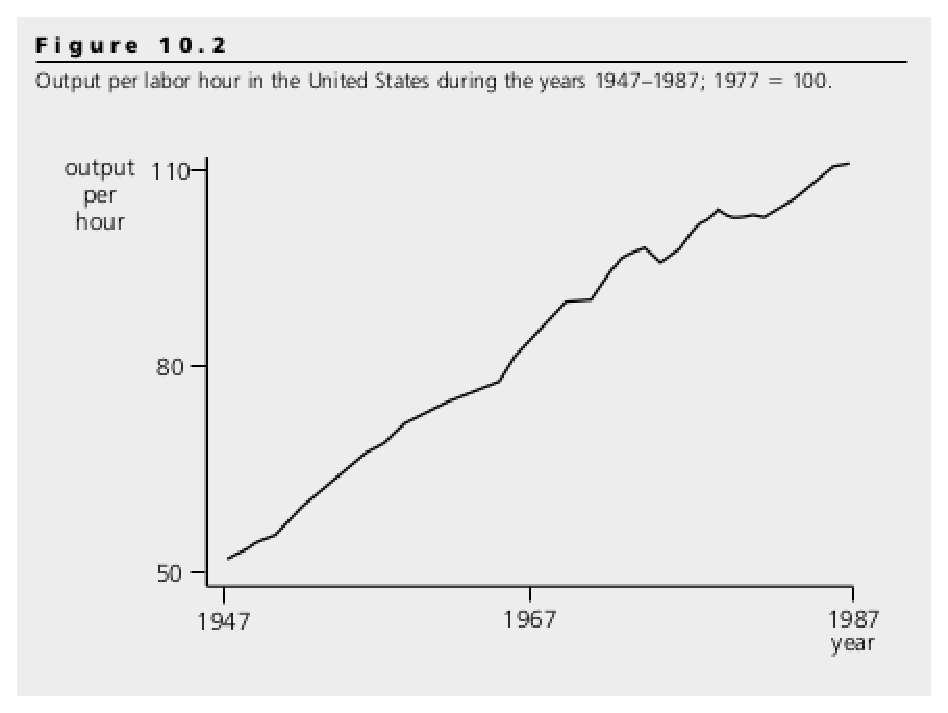
\includegraphics[scale = 0.5]{pictures/figure_10_2.eps}
\caption{Časová řada s lineárním trendem}
\label{figure_10_2}
\end{figure}

Mnoho časových řad je charakteristických exponenciálním trendem, 
což znamená konstantní relativní změnu v čase. V praxi 
exponenciální trend často podchycujeme pomocí modelu
\begin{equation}
\log(y_t) = \beta_0 + \beta_1 t + e_t, ~~~ t = 1, 2, ...,
\end{equation}
kde $\beta_1$ označujeme jako míru růstu $y$.

\begin{figure}[htp]
\centering
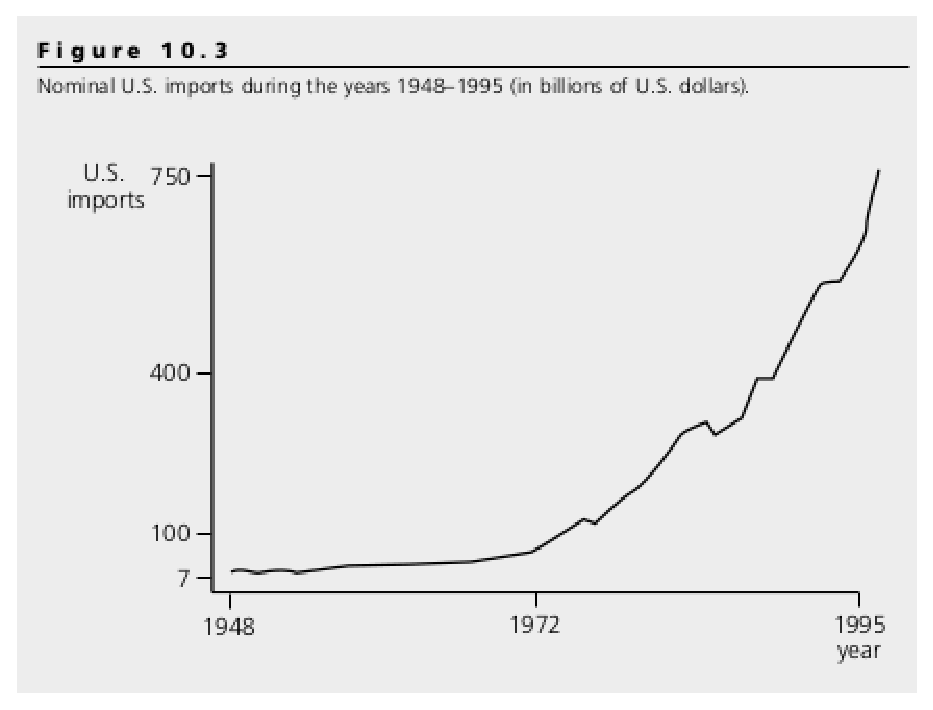
\includegraphics[scale = 0.5]{pictures/figure_10_3.eps}
\caption{Časová řada s exponenciálním trendem}
\label{figure_10_3}
\end{figure}

Ačkoliv lineární a exponenciální trendy jsou nejběžnější, 
můžeme se občas setkat také komplikovanějšími časovými trendy. Jako příklad uveďme 
model s kvadratickým trendem
\begin{equation}
y_t = \alpha_0 + \alpha_1 t + \alpha_2 t^2 + e_t,
\end{equation}
který je vhodný např. pro časové řady, ve kterých je rostoucí 
trend následovaný klesajícím trendem.

\subsubsection{Časové trendy a zdánlivá korelace}

Trendové proměnné neporušují žádný z předpokladů TS.1 až 
TS.6. Nicméně je důležité si uvědomit, že skryté faktory, 
které způsobují trend v $y$, mohou být také korelovány s 
nezávislými veličinami. Pokud bychom toto nebrali v potaz, 
vystavovali bychom se riziku tzv. zavádějící korelace (spurious 
correlation), kdy zdánlivá souvislost mezi dvěma náhodnými 
veličinami je dána pouze tím, je obě sledují obdobný trend. 
Přidáním časového trendu do modelu lze tento problém snadno eliminovat.

Pro ilustraci uvažujme nezávislé veličiny $x_{t1}$ a $x_{t2}$, 
které sledují lineární trend, a model
\begin{equation}
y_t = \beta_0 + \beta_1 x_{t1} + \beta_2 x_{t2} + \beta_3 t + u_t.
\end{equation}
Tento model zapadá do obecné metodologie vícerozměrného 
regresního modelu, protože $t$ můžeme chápat jako další 
nezávislou veličinu, tj. $t = x_{t3}$. Díky zohlednění 
časového trendu v modelu může $y_t$ lineárně růst popř. klesat 
v čase. Jestliže výše uvedený model splňuje předpoklady TS.1 až 
TS.3, pak vynechání $t$ z regresního modelu má za následek 
zkreslené odhady parametrů $\beta_1$ a $\beta_2$ v důsledku 
vynechání relevantní vysvětlující proměnné.

\subsubsection{Interpretace sklonu regresního modelu a odstranění trendu}

Jestliže (stejně jako ve výše uvedeném příkladě) provádíme regresi 
$y_i$ na $x_{t1}$, $x_{t2}$ a $t$, získáme odhad modelu ve tvaru
\begin{equation}
\hat{y}_t = \hat{\beta}_0 + \hat{\beta}_1 x_{t1} + \hat{\beta}_{t2} + 
\hat{\beta}_3 t.
\end{equation}

Odhady $\hat{\beta}_1$ a $\hat{\beta}_2$ však lze získat také 
následujícím způsobem. Nejprve provedeme regresi $y_t$, $x_{t1}$ a $x_{t2}$ na konstantu a 
časový trend $t$, čímž získáme rezidua $\ddot{y}_t$, 
$\ddot{x}_{t1}$ a $\ddot{x}_{t2}$ pro $t = 1, 2, ..., n$, např.
\begin{equation}
\ddot{y}_t = y_t - \hat{\alpha}_0 + \hat{\alpha}_1 t.
\end{equation}
O $\ddot{y}_t$ můžeme uvažovat jako o veličině, ze které jsme 
odstranili lineární trend. Pro odstranění trendu jsme museli nejprve
odhadnout model
\begin{equation}
y_t = \alpha_0 + \alpha_1 t + e_t
\end{equation}
pomocí OLS; rezidua z této regrese, tj. $\hat{e}_t = \ddot{y}_t$, 
jsou zbavené případného lineárního trendu. Podobná interpretace 
platí také pro $\ddot{x}_{t1}$ a $\ddot{x}_{t2}$.

Následně provedeme regresi $\ddot{y}_t$ na $\ddot{x}_{t1}$ a 
$\ddot{x}_{t2}$.\footnote{Do regresního modelu není třeba není 
třeba zahrnout průsečík. Pokud ho zahrneme, bude odhadnut na nulu.} 
Odhady sklonů tohoto regresního modelu budou odpovídat odhadům 
sklonů regresního modelu (10.31). To znamená, že odhady sklonu z 
(10.31) můžeme interpretovat jako odhady po odstranění lineárního 
trendu. Analogicky můžeme postupovat také v případě vícero 
vysvětlujících veličin či v případě exponenciálního či 
kvadratického trendu.

Pokud bychom z modelu (10.31) odstranili $t$ jako nezávislou 
veličinu, k odstranění trendu by nedošlo. Pak by se mohlo zdát, 
že na vývoj $y_t$ má vliv jedno či vícero $x_{tj}$. To by však 
mohlo být způsobeno pouze tím, že všechny tyto veličiny zahrnují 
časový trend.

Interpretace $\hat{\beta}_1$ a $\hat{\beta}_2$ ukazuje, že je vhodné 
zahrnout časový trend do regresního modelu, jestliže některá z 
nezávislých veličin sleduje trend, i když $y_t$ v sobě trend 
neobsahuje. V opačném případě by se totiž mohlo stát, že by 
vysvětlující veličina nevykazovala vazbu na $y_t$, ačkoliv by 
její pohyb okolo trendu na vývoj $y_t$ vliv měl.

\subsubsection{Výpočet $R^2$ v případě, že závislá veličina 
sleduje trend}

Při porovnání s modely založenými na průřezových datech je $R^2$ regresních modelů časových řad často velmi 
vysoké.
To může být způsobeno tím, že závislá veličina sleduje 
časový trend. Připomeňme, že
\begin{equation}
\bar{R}^2 = 1 - \frac{\hat{\sigma}^2_u}{\hat{\sigma}^2_y},
\end{equation}
kde $\hat{\sigma}^2_u$ je nestranná funkce odhadu rozptylu chyby 
regresního modelu a $\hat{\sigma}^2_y = \frac{SST}{n - 1} = 
\frac{\sum_{t = 1}^n(y_t - \bar{y})^2}{n - 1}$. Jestliže $E[y_t]$ 
sleduje např. lineární trend, pak $\frac{SST}{n - 1}$ není 
nestranná a konzistentní funkce odhadu $var[y_t]$. Ve skutečnosti 
může $\frac{SST}{n - 1}$ výrazným způsobem nadhodnocovat rozptyl 
$y_t$, protože nezohledňuje trend obsažený v $y_t$.

Nejjednodušším řešením je vypočíst $R^2$ po té, co byl ze 
závislé veličiny odstraněn trend, tj. jako
\begin{equation}
R^2 = 1 - \frac{\hat{\sigma}^2_u}{\sum_{t = 1}^n \ddot{y}_t^2}.
\end{equation}
Protože $\sum_{t = 1}^n \ddot{y}_t^2 \le \sum_{t = 1}^n (y_t - 
\bar{y})^2$, platí $R^2 \le \bar{R}^2$. Pokud $y_t$ obsahuje silný 
trend, může být $R^2$ výrazně nižší než $\bar{R}^2$. $R^2$ tak
lépe vysvětluje, jak je $y_t$ ovlivněno $x_{t1}$ a $x_{t2}$, 
protože zohledňuje případnou existenci časového trendu.

Korigované $R^2$ lze vypočíst analogicky dle (10.35) s tím, že 
$\hat{\sigma}^2_u$ vydělíme $n - 4$, protože to je počet stupňů 
volnosti v (10.31), a $\sum_{t = 1}^n \ddot{y}_t^2$ vydělíme $n - 2$, 
protože při odstranění trendu z $y_1$ pomocí (10.33) odhadujeme dva parametry.

Závěrem bychom měli zdůraznit, že při výpočtu $R^2$ formy $F$ statistiky pro účely testování vícero 
lineárních omezení používáme klasické $R^2$ bez odstranění 
trendu. Důvodem je, že $R^2$ forma $F$ statistiky je pouze 
výpočetní nástroj, a proto je žádoucí použít klasickou formu $R^2$.

\subsubsection{Sezónnost}

Mnoho časových řady vykazuje známky tzv. sezónností. Sezónnost chápeme 
jako situaci, kdy je časová řada výrazným způsobem 
ovlivněna aktuálním měsícem popř. ročním obdobím. Za časové 
řady, které vykazují znaky sezónnosti, můžeme považovat např. 
výnosy v zemědělství nebo počet udělených stavebních povolení. 
Některé řady mohou obsahovat jak časový trend, tak sezónnost - 
typickým příkladem takovéto řady je např. vývoj HDP.

Z časových řad, které jsou publikované statistickými úřady, je 
sezónnost velice často odstraněna. Existuje mnoho způsobů, jak z 
časové řady sezónnost odstranit, nicméně detailní popis odpovídajících 
postupů překračuje záběr této knihy. Proto si vysvětlíme pouze 
jednu relativně přímočarou metodu.

Nejjednodušším způsobem, jak odstranit sezónnost z časové řady, je pomocí 
binárních veličin. Předpokládejme, že máme k dispozici 
měsíční data, a uvažujme následující regresní model
\begin{multline}
y_t = \beta_0 + \delta_1 feb_t + \delta_2 mar_t + \delta_3 apr_t + 
...\\ 
+ \delta_{11} dec_t + \beta_1 x_{t1} + ... + \beta_k x_{tk} + u_t,
\end{multline}
kde $feb_t$, $mar_t$, ..., $dec_t$ představují binární veličiny, 
které indikují kalendářní měsíc dané časové periody 
$t$.\footnote{Měsíc leden byl záměrně vynechán, abychom se 
vyhnuli tzv. pasti binární veličiny.} 
Pokud $y_t$ nevykazuje sezónnost, pak jsou $\delta_1$ až $\delta_{11}$ 
sdruženě statisticky nevýznamné, což lze otestovat pomocí $F$ 
statistiky. Analogicky lze postupovat, pokud máme k dispozici 
čtvrtletní namísto měsíčních dat.

Sezónnost lze z časových řad odstranit podobným způsobem, jakým 
jsme odstranily trend. Uvažujme rovnici (10.36) s $k = 2$. Odhady 
$\hat{\beta}_1$ a $\hat{\beta}_2$ lze získat následovně.

Nejprve provedeme regresi $y_t$, $x_{t1}$ a $x_{t2}$ na konstantu a 
binární veličiny reprezentující měsíce únor až prosinec, 
abychom získali rezidua $\ddot{y}_t$, $\ddot{x}_{t1}$ a 
$\ddot{x}_{t2}$ pro všechna $t = 1, 2, ..., n$. Jako příklad uveďme
\begin{equation}
\ddot{y}_t = y_t - \hat{\alpha}_0 - \hat{\alpha}_1 feb_t - 
\hat{\alpha}_2 mar_t - ... - \hat{\alpha}_{11} dec_t,
\end{equation}
čímž jsme odstranili sezónnost z měsíční časové řady $y_t$. 
Podobnou interpretaci lze použít také v případě časových řad 
$\ddot{x}_{t1}$ a $\ddot{x}_{t2}$. Následně provedeme regresi $\ddot{y}_t$ na $\ddot{x}_{t1}$ a 
$\ddot{x}_{t2}$, čímž získáme odhady $\hat{\beta}_1$ a $\hat{\beta}_2$.

V případě, že $y_t$ vykazuje silné známky sezónnosti, je vhodné tuto skutečnost zohlednit v $R^2$ podobně, jak tomu bylo v případě časového trendu. Tímto způsobem se zbavíme sezónních vlivů, které nejsou vysvětleny pomocí $x_{tj}$.

Jak jsme již dříve zmínili, mnoho časových řad vykazuje známky 
jak časového trendu, tak sezónnosti. V takovémto případě by 
regresní model měl zahrnovat časový trend i sezónní 
binární veličiny.
